\chapter{Matrix Decompositions: Breaking Things to Understand Them Better}

% ============================================
% TikZ Style Definitions - Simple and Readable (matching Chapter 1)
% ============================================
\tikzset{
    % Axis styles - dark enough to read
    axis/.style={->, thick, black!60},
    axis label/.style={font=\footnotesize, black!70},
    % Grid styles
    grid/.style={very thin, black!15},
    % Vector styles - bold colors
    vec blue/.style={->, very thick, blue!80!black},
    vec red/.style={->, very thick, red!70!black},
    vec green/.style={->, very thick, green!50!black},
    vec purple/.style={->, very thick, purple!70!black},
    vec orange/.style={->, very thick, orange!70!black},
    % Label styles - simple and readable
    vec label/.style={font=\footnotesize},
    title label/.style={font=\footnotesize\bfseries},
    % Dashed helper lines
    helper/.style={dashed, black!40, thin},
}

\section{The IKEA Philosophy of Mathematics}

\subsection{Why Breaking Things Apart Is Actually Smart}

You know what IKEA figured out that made them billions of dollars? Shipping fully assembled furniture is expensive and inefficient. A fully built wardrobe? Good luck fitting that in your car. But if you break a bookshelf into flat pieces, suddenly you can fit 50 of them in one truck. Genius!

Matrix decompositions are the same idea, except instead of making shipping easier, they make computation faster, storage cheaper, and understanding deeper. And unlike IKEA furniture, you won't end up with mysterious leftover screws.

\textbf{The core insight:} A big complicated matrix can often be broken into a product of simpler matrices. And once it's broken apart, you can:
\begin{itemize}
    \item Store it more efficiently (compression!)
    \item Compute with it faster (optimization!)
    \item Understand what it's doing (interpretation!)
    \item Fix parts without rebuilding everything (adaptation!)
\end{itemize}

\begin{intuition}
Think of a matrix decomposition like this:

\textbf{Before:} "This 1000×1000 matrix does... something complicated. It has a million numbers in it. Good luck understanding it, buddy."

\textbf{After:} "Oh! It's actually just a rotation ($\mat{Q}$) followed by a stretch ($\mat{D}$) followed by another rotation ($\mat{Q}^\top$). Now I get it! It's like a cosmic yoga pose for vectors!"

Decompositions turn mysterious black boxes into transparent, modular components. It's like opening up a magic trick and seeing there's just three simple steps that create the illusion.
\end{intuition}

\subsection{A Real-World Analogy: The Recipe Book}

Imagine you have a super complicated recipe for a fancy wedding cake. It's 47 steps long, uses 23 ingredients, and takes 6 hours. Terrifying, right?

But what if I told you it's actually just:
\begin{enumerate}
    \item Make a basic vanilla cake (you know how to do this!)
    \item Make buttercream frosting (easy peasy!)
    \item Stack them and decorate (the fun part!)
\end{enumerate}

Each piece is simple. The combination creates something impressive. That's exactly what matrix decomposition does—it breaks scary math into friendly, bite-sized pieces.

\begin{connection}
\textbf{Why LLMs love decompositions (and why you should too):}

GPT-3 has \textbf{175 billion parameters}. That's 175,000,000,000 numbers. If you printed them out, you'd need about 35 million pages. That's a LOT of numbers to store and compute with.

Decompositions let us:
\begin{itemize}
    \item \textbf{Compress models:} Store a 4096×4096 matrix as two 4096×64 matrices. That's like compressing a library into a pamphlet! (This is called LoRA, and it's magical.)
    \item \textbf{Speed up inference:} Compute faster by exploiting structure. Your chatbot responds quicker!
    \item \textbf{Fine-tune efficiently:} Update only small low-rank pieces instead of everything. Like renovating your kitchen instead of rebuilding your house.
    \item \textbf{Understand attention:} Decompose attention matrices to see what patterns the model learned.
\end{itemize}

Let's learn the main decompositions and why they matter!
\end{connection}

\section{Cholesky Decomposition: The Matrix Square Root}

\subsection{Taking the Square Root of a Matrix (Yes, Really!)}

Remember in elementary school when you learned that $5^2 = 25$, so $\sqrt{25} = 5$? You were basically taught that some operations can be reversed. Squaring has a reverse called square rooting.

Here's a wild thought: \textbf{What if we could do the same thing for matrices?}

Spoiler alert: We can! And it's called the Cholesky decomposition. (Named after André-Louis Cholesky, a French military officer who did math in his spare time because apparently fighting in WWI wasn't exciting enough.)

\textbf{The setup:} You have a special kind of matrix $\mat{A}$ that's:
\begin{itemize}
    \item \textbf{Symmetric:} $\mat{A} = \mat{A}^\top$ (it's a mirror image across the diagonal—like a butterfly's wings)
    \item \textbf{Positive definite:} $\vect{x}^\top \mat{A} \vect{x} > 0$ for all non-zero $\vect{x}$
\end{itemize}

\textbf{Wait, what does "positive definite" even mean?}

Great question! Think of it like this: Imagine you're standing at the bottom of a bowl (like a salad bowl, not a Super Bowl). No matter which direction you walk, you go uphill. That's positive definite—it curves upward in \textit{every} direction.

A negative definite matrix is like standing on a dome—every direction goes downhill. An indefinite matrix is like a saddle—some directions go up, some go down.

\begin{center}
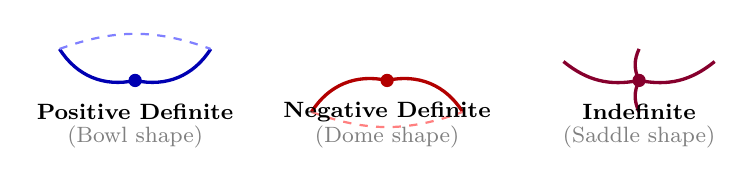
\begin{tikzpicture}[scale=0.8]
    % Positive definite - bowl
    \begin{scope}
        \draw[very thick, blue!70!black] (-1.2,0.5) to[bend right=35] (0,0) to[bend right=35] (1.2,0.5);
        \draw[thick, blue!50, dashed] (-1.2,0.5) to[bend left=20] (1.2,0.5);
        \fill[blue!70!black] (0,0) circle (3pt);
        \node[font=\footnotesize\bfseries] at (0,-0.5) {Positive Definite};
        \node[font=\footnotesize, gray] at (0,-0.9) {(Bowl shape)};
    \end{scope}

    % Negative definite - dome
    \begin{scope}[xshift=4cm]
        \draw[very thick, red!70!black] (-1.2,-0.5) to[bend left=35] (0,0) to[bend left=35] (1.2,-0.5);
        \draw[thick, red!50, dashed] (-1.2,-0.5) to[bend right=20] (1.2,-0.5);
        \fill[red!70!black] (0,0) circle (3pt);
        \node[font=\footnotesize\bfseries] at (0,-0.5) {Negative Definite};
        \node[font=\footnotesize, gray] at (0,-0.9) {(Dome shape)};
    \end{scope}

    % Indefinite - saddle
    \begin{scope}[xshift=8cm]
        \draw[very thick, purple!70!black] (-1.2,0.3) to[bend right=25] (0,0) to[bend right=25] (1.2,0.3);
        \draw[very thick, purple!70!black] (0,0.5) to[bend right=25] (0,0) to[bend right=25] (0,-0.5);
        \fill[purple!70!black] (0,0) circle (3pt);
        \node[font=\footnotesize\bfseries] at (0,-0.5) {Indefinite};
        \node[font=\footnotesize, gray] at (0,-0.9) {(Saddle shape)};
    \end{scope}
\end{tikzpicture}
\end{center}

Positive definite matrices show up everywhere in machine learning, especially when dealing with covariances (how things vary together), Hessians (second derivatives in optimization), and kernel matrices (similarity measures).

\begin{definition}{Cholesky Decomposition}{}
For a positive definite matrix $\mat{A}$, there exists a \textbf{unique} lower triangular matrix $\mat{L}$ such that:
\[
\mat{A} = \mat{L} \mat{L}^\top
\]

We call $\mat{L}$ the \vocab{Cholesky factor} of $\mat{A}$.

\textbf{In plain English:} "$\mat{L}$ is like the square root of $\mat{A}$ because $\mat{L}$ times its transpose gives you $\mat{A}$."

It's like saying: "What matrix, when multiplied by its own reflection, gives us back $\mat{A}$?" And the answer is $\mat{L}$!
\end{definition}

\textbf{What's a lower triangular matrix?}

It's a matrix where everything \textit{above} the diagonal is zero. Like a staircase going down:

\[
\mat{L} = \begin{bmatrix}
\text{something} & 0 & 0 \\
\text{something} & \text{something} & 0 \\
\text{something} & \text{something} & \text{something}
\end{bmatrix}
\]

The zeros above the diagonal make these matrices super easy to work with. Solving equations with triangular matrices is like unwrapping a present one layer at a time—each step reveals the next.

\vspace{0.3cm}
\begin{center}
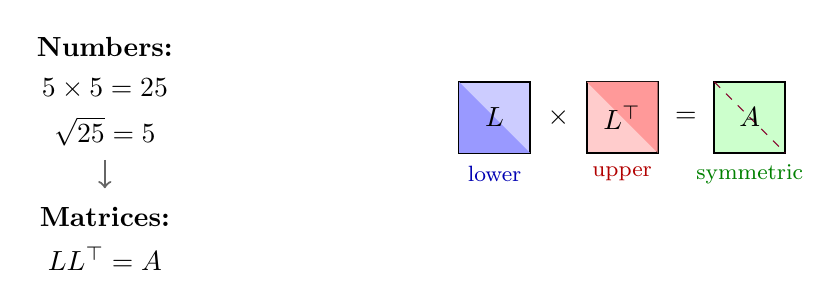
\begin{tikzpicture}[scale=0.9]
    % Left side: concept
    \node[font=\bfseries] at (0,1.5) {Numbers:};
    \node at (0,0.9) {$5 \times 5 = 25$};
    \node at (0,0.3) {$\sqrt{25} = 5$};

    \draw[->, thick, black!60] (0,-0.1) -- (0,-0.5);

    \node[font=\bfseries] at (0,-0.9) {Matrices:};
    \node at (0,-1.5) {$\mat{L} \mat{L}^\top = \mat{A}$};

    % Right side: visual
    \begin{scope}[xshift=5cm]
        % L matrix (lower triangular)
        \draw[thick, fill=blue!20] (0,0) rectangle (1,1);
        \fill[blue!40] (0,0) -- (0,1) -- (1,0) -- cycle;
        \node at (0.5,0.5) {$\mat{L}$};
        \node[font=\footnotesize, blue!70!black] at (0.5,-0.3) {lower};

        \node at (1.4,0.5) {$\times$};

        % L^T matrix (upper triangular)
        \draw[thick, fill=red!20] (1.8,0) rectangle (2.8,1);
        \fill[red!40] (1.8,1) -- (2.8,1) -- (2.8,0) -- cycle;
        \node at (2.3,0.5) {$\mat{L}^\top$};
        \node[font=\footnotesize, red!70!black] at (2.3,-0.3) {upper};

        \node at (3.2,0.5) {$=$};

        % A matrix (symmetric)
        \draw[thick, fill=green!20] (3.6,0) rectangle (4.6,1);
        \draw[dashed, purple!70!black] (3.6,1) -- (4.6,0);
        \node at (4.1,0.5) {$\mat{A}$};
        \node[font=\footnotesize, green!50!black] at (4.1,-0.3) {symmetric};
    \end{scope}
\end{tikzpicture}
\end{center}
\vspace{0.3cm}

\subsection{Let's Actually Do One! (Don't Panic)}

I know what you're thinking: "This sounds complicated." But it's actually not! Let's work through an example step by step, like following a recipe.

\begin{example}
Let's find the Cholesky decomposition of:
\[
\mat{A} = \begin{bmatrix}
4 & 2 \\
2 & 3
\end{bmatrix}
\]

\textbf{First, let's verify this is positive definite:}
\begin{itemize}
    \item It's symmetric? \checkmark{} (2 appears in both off-diagonal spots)
    \item The diagonal entries are positive? \checkmark{} (4 and 3 are both positive)
    \item Determinant is positive? $4 \times 3 - 2 \times 2 = 12 - 4 = 8 > 0$ \checkmark{}
\end{itemize}

Great! We can proceed. (If any of these failed, there would be no Cholesky decomposition—like trying to take the square root of a negative number.)

\textbf{Now, we want to find $\mat{L}$ such that:}
\[
\begin{bmatrix}
4 & 2 \\
2 & 3
\end{bmatrix}
= \begin{bmatrix}
\ell_{11} & 0 \\
\ell_{21} & \ell_{22}
\end{bmatrix}
\begin{bmatrix}
\ell_{11} & \ell_{21} \\
0 & \ell_{22}
\end{bmatrix}
\]

Notice how $\mat{L}^\top$ is just $\mat{L}$ flipped across the diagonal? The zeros switch from bottom-left to top-right.

\textbf{Step 1: Multiply out the right side}

Let's do the matrix multiplication:
\[
\mat{L}\mat{L}^\top = \begin{bmatrix}
\ell_{11} \cdot \ell_{11} + 0 \cdot 0 & \ell_{11} \cdot \ell_{21} + 0 \cdot \ell_{22} \\
\ell_{21} \cdot \ell_{11} + \ell_{22} \cdot 0 & \ell_{21} \cdot \ell_{21} + \ell_{22} \cdot \ell_{22}
\end{bmatrix}
= \begin{bmatrix}
\ell_{11}^2 & \ell_{11}\ell_{21} \\
\ell_{11}\ell_{21} & \ell_{21}^2 + \ell_{22}^2
\end{bmatrix}
\]

\textbf{Step 2: Match components (like a puzzle!)}

Now we just match up corresponding entries:

\begin{itemize}
    \item \textbf{Top-left:} $\ell_{11}^2 = 4$

    What number squared gives 4? That's $\ell_{11} = 2$ (we take the positive root)

    \item \textbf{Top-right (or bottom-left, they're equal):} $\ell_{11}\ell_{21} = 2$

    We know $\ell_{11} = 2$, so $2 \cdot \ell_{21} = 2$, which means $\ell_{21} = 1$

    \item \textbf{Bottom-right:} $\ell_{21}^2 + \ell_{22}^2 = 3$

    We know $\ell_{21} = 1$, so $1 + \ell_{22}^2 = 3$, which means $\ell_{22}^2 = 2$, so $\ell_{22} = \sqrt{2}$
\end{itemize}

\textbf{Step 3: Assemble the answer!}
\[
\mat{L} = \begin{bmatrix}
2 & 0 \\
1 & \sqrt{2}
\end{bmatrix}
\]

\textbf{Step 4: Let's double-check (always a good idea!)}
\[
\begin{bmatrix}
2 & 0 \\
1 & \sqrt{2}
\end{bmatrix}
\begin{bmatrix}
2 & 1 \\
0 & \sqrt{2}
\end{bmatrix}
= \begin{bmatrix}
4 & 2 \\
2 & 1 + 2
\end{bmatrix}
= \begin{bmatrix}
4 & 2 \\
2 & 3
\end{bmatrix}
\]

\textbf{Perfect!} \checkmark{} We found the matrix square root!
\end{example}

\begin{intuition}
\textbf{Why did that work?}

We essentially "built up" the matrix from scratch. Starting from the top-left corner, we figured out each entry one at a time. The triangular structure meant each new entry only depended on things we'd already computed.

It's like solving a Sudoku where each number you fill in reveals the next one!
\end{intuition}

\subsection{Why This Is Ridiculously Useful (The Practical Magic)}

"Okay," you say, "I can find the Cholesky factor. But why would I want to?"

Great question! Here are three killer applications:

\vspace{0.3cm}
\textbf{Application 1: Solving Systems of Equations FAST}

Suppose you need to solve $\mat{A}\vect{x} = \vect{b}$ (find $\vect{x}$ given $\mat{A}$ and $\vect{b}$).

\textbf{The slow way:} Compute $\mat{A}^{-1}$ and multiply: $\vect{x} = \mat{A}^{-1}\vect{b}$. This is expensive and can be numerically unstable.

\textbf{The Cholesky way:} Since $\mat{A} = \mat{L}\mat{L}^\top$, we rewrite as $\mat{L}\mat{L}^\top\vect{x} = \vect{b}$

Now split it into two easy problems:
\begin{enumerate}
    \item Solve $\mat{L}\vect{y} = \vect{b}$ for $\vect{y}$ (easy—$\mat{L}$ is lower triangular!)
    \item Solve $\mat{L}^\top\vect{x} = \vect{y}$ for $\vect{x}$ (also easy—$\mat{L}^\top$ is upper triangular!)
\end{enumerate}

\textbf{Why is triangular easy?} Because you can solve it one row at a time!

For a lower triangular system:
\begin{align}
2x_1 &= 6 \quad \Rightarrow \quad x_1 = 3 \quad \text{(just divide!)} \nonumber \\
x_1 + 3x_2 &= 9 \quad \Rightarrow \quad 3 + 3x_2 = 9 \quad \Rightarrow \quad x_2 = 2 \quad \text{(substitute and solve!)} \nonumber
\end{align}

Each row only involves the variables you've already found, plus one new one. It's like a ladder—climb one rung at a time!

\textbf{Speed comparison:} For an $n \times n$ matrix:
\begin{itemize}
    \item General solver: About $n^3$ operations
    \item Cholesky + triangular solves: About $\frac{1}{3}n^3$ operations for factoring, then $n^2$ per solve
\end{itemize}

If you need to solve many systems with the same $\mat{A}$ but different $\vect{b}$ vectors (common in practice!), Cholesky is a huge win. Factor once, solve cheaply many times!

\vspace{0.3cm}
\textbf{Application 2: Generating Random Samples (Making Randomness Correlated)}

This one's cool. Suppose you want to generate random samples from a multivariate Gaussian distribution $\mathcal{N}(\vect{\mu}, \mat{\Sigma})$.

\textbf{The problem:} You can easily generate independent random numbers (like rolling dice). But what if you want correlated random numbers (like height and weight, which tend to go together)?

\textbf{The Cholesky solution:}

\begin{enumerate}
    \item Compute Cholesky: $\mat{\Sigma} = \mat{L}\mat{L}^\top$
    \item Sample independent standard normals: $\vect{z} \sim \mathcal{N}(\vect{0}, \mat{I})$ (just random numbers, uncorrelated)
    \item Transform: $\vect{x} = \vect{\mu} + \mat{L}\vect{z}$
\end{enumerate}

Now $\vect{x}$ has the exact right mean and covariance!

\textbf{What's happening intuitively?} $\mat{L}$ is like a "correlation machine." You feed in independent randomness, and it mixes them together to create the right correlations.

Imagine you have two random number generators: one for "general health" and one for "exercise amount." $\mat{L}$ says: "To get height, take 90\% of health and 10\% of exercise. To get weight, take 80\% of health and 20\% of exercise." Now height and weight are correlated!

\vspace{0.3cm}
\textbf{Application 3: Checking if a Matrix is "Valid"}

Sometimes you compute a covariance matrix and wonder: "Is this actually a valid covariance matrix?"

A valid covariance matrix must be positive semi-definite (the bowl shape we discussed). A quick test:

\begin{enumerate}
    \item Try to compute the Cholesky decomposition
    \item If it works \textrightarrow{} Valid! \checkmark{}
    \item If you get a negative number under a square root \textrightarrow{} Invalid! $	imes$
\end{enumerate}

It's like a "positive definiteness detector." Very handy!

\begin{connection}
\textbf{In machine learning, Cholesky is everywhere:}

\textbf{Gaussian Processes:} These powerful models for regression and uncertainty quantification use covariance matrices extensively. Cholesky is the workhorse for all computations!

\textbf{Optimization (Newton's Method):} When you're optimizing a function, you often need to use second derivatives (the Hessian matrix). If it's positive definite, Cholesky gives you a fast, stable way to take steps.

\textbf{Variational Autoencoders (VAEs):} These generative models need to sample from Gaussian distributions—hello, Cholesky!

\textbf{Bayesian Deep Learning:} When estimating uncertainty in neural networks, you often work with covariance matrices of weights. Cholesky makes this tractable.
\end{connection}

\section{LU Decomposition: The Systematic Eliminator}

\subsection{Remember Gaussian Elimination from School?}

Pop quiz: In high school algebra, how did you solve systems of equations?

If you said "Gaussian elimination" (or "that thing where you add and subtract rows to make zeros"), congratulations! You already understand LU decomposition. It's just that process, gift-wrapped in a fancy matrix package!

\textbf{The basic idea:} Take any matrix (doesn't need to be symmetric or positive definite—any square matrix works!) and break it into two triangular matrices.

\begin{definition}{LU Decomposition}{}
For a matrix $\mat{A}$, we can write:
\[
\mat{A} = \mat{L}\mat{U}
\]

where:
\begin{itemize}
    \item $\mat{L}$ is \textbf{L}ower triangular (zeros above diagonal)—the "multipliers" from elimination
    \item $\mat{U}$ is \textbf{U}pper triangular (zeros below diagonal)—the "end result" after elimination
\end{itemize}

Sometimes we need to swap rows first (called "pivoting"), so we write:
\[
\mat{P}\mat{A} = \mat{L}\mat{U}
\]

where $\mat{P}$ is a permutation matrix (it just swaps rows around—no actual math, just rearranging).
\end{definition}

\textbf{Why "LU"?} Because mathematicians are very creative with names. L for Lower, U for Upper. Groundbreaking stuff.

\subsection{Let's Do Gaussian Elimination (And Watch LU Appear!)}

\begin{example}
Let's decompose this matrix:
\[
\mat{A} = \begin{bmatrix}
2 & 1 & 1 \\
4 & 3 & 3 \\
8 & 7 & 9
\end{bmatrix}
\]

\textbf{Goal:} Turn this into an upper triangular matrix by making zeros below the diagonal.

\textbf{Step 1: Eliminate the first column (below the diagonal)}

Look at position (2,1). It has a 4, but we want a 0.

How do we make it zero? Row 2 minus 2 times Row 1:
\[
\begin{bmatrix} 4 & 3 & 3 \end{bmatrix} - 2 \times \begin{bmatrix} 2 & 1 & 1 \end{bmatrix} = \begin{bmatrix} 0 & 1 & 1 \end{bmatrix}
\]

\textbf{Important:} Remember that multiplier (2)! We'll need it later.

Now our matrix looks like:
\[
\begin{bmatrix}
2 & 1 & 1 \\
0 & 1 & 1 \\
8 & 7 & 9
\end{bmatrix}
\]

Next, position (3,1) has an 8. We want zero.

Row 3 minus 4 times Row 1:
\[
\begin{bmatrix} 8 & 7 & 9 \end{bmatrix} - 4 \times \begin{bmatrix} 2 & 1 & 1 \end{bmatrix} = \begin{bmatrix} 0 & 3 & 5 \end{bmatrix}
\]

\textbf{Remember that multiplier too (4)!}

Now:
\[
\begin{bmatrix}
2 & 1 & 1 \\
0 & 1 & 1 \\
0 & 3 & 5
\end{bmatrix}
\]

First column is done! \checkmark{}

\textbf{Step 2: Eliminate the second column (below the diagonal)}

Position (3,2) has a 3. We want zero.

Row 3 minus 3 times Row 2:
\[
\begin{bmatrix} 0 & 3 & 5 \end{bmatrix} - 3 \times \begin{bmatrix} 0 & 1 & 1 \end{bmatrix} = \begin{bmatrix} 0 & 0 & 2 \end{bmatrix}
\]

\textbf{Multiplier: 3}

Final result:
\[
\mat{U} = \begin{bmatrix}
2 & 1 & 1 \\
0 & 1 & 1 \\
0 & 0 & 2
\end{bmatrix}
\]

This is our $\mat{U}$—upper triangular!

\textbf{Step 3: Build $\mat{L}$ from the multipliers}

Remember all those multipliers we saved? (2, 4, 3)

They go into $\mat{L}$ in the exact positions where we created zeros:
\[
\mat{L} = \begin{bmatrix}
1 & 0 & 0 \\
2 & 1 & 0 \\
4 & 3 & 1
\end{bmatrix}
\]

The diagonal is all 1s (we didn't modify the diagonal), and the multipliers fill in below.

\textbf{Step 4: Verify!}
\[
\mat{L}\mat{U} = \begin{bmatrix}
1 & 0 & 0 \\
2 & 1 & 0 \\
4 & 3 & 1
\end{bmatrix}
\begin{bmatrix}
2 & 1 & 1 \\
0 & 1 & 1 \\
0 & 0 & 2
\end{bmatrix}
= \begin{bmatrix}
2 & 1 & 1 \\
4 & 3 & 3 \\
8 & 7 & 9
\end{bmatrix}
= \mat{A}
\]

It works! \checkmark{}
\end{example}

\vspace{0.3cm}
\begin{center}
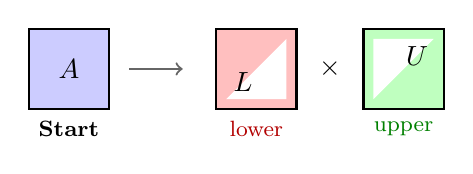
\begin{tikzpicture}[scale=0.85]
    % Start: Full matrix A
    \draw[thick, fill=blue!20] (0,0) rectangle (1.2,1.2);
    \node at (0.6,0.6) {$\mat{A}$};
    \node[font=\footnotesize\bfseries] at (0.6,-0.3) {Start};

    % Arrow
    \draw[->, thick, black!60] (1.5,0.6) -- (2.3,0.6);

    % Result: L and U
    \begin{scope}[xshift=2.8cm]
        % L matrix (lower triangular)
        \draw[thick, fill=red!25] (0,0) rectangle (1.2,1.2);
        \fill[white] (0.15,0.15) -- (1.05,0.15) -- (1.05,1.05) -- cycle;
        \draw[thick] (0,0) rectangle (1.2,1.2);
        \node at (0.4,0.4) {$\mat{L}$};
        \node[font=\footnotesize, red!70!black] at (0.6,-0.3) {lower};
    \end{scope}

    \node at (4.5,0.6) {$\times$};

    \begin{scope}[xshift=5cm]
        % U matrix (upper triangular)
        \draw[thick, fill=green!25] (0,0) rectangle (1.2,1.2);
        \fill[white] (0.15,0.15) -- (0.15,1.05) -- (1.05,1.05) -- cycle;
        \draw[thick] (0,0) rectangle (1.2,1.2);
        \node at (0.8,0.8) {$\mat{U}$};
        \node[font=\footnotesize, green!50!black] at (0.6,-0.3) {upper};
    \end{scope}
\end{tikzpicture}
\end{center}

\noindent\textit{The diagram shows: Full matrix $\rightarrow$ eliminate to get upper triangular $\mat{U}$, save multipliers in lower triangular $\mat{L}$.}
\vspace{0.3cm}

\begin{intuition}
\textbf{What's the deep meaning here?}

$\mat{L}$ and $\mat{U}$ together encode \textbf{both the answer and the process}!

Think of it like a cooking show:
\begin{itemize}
    \item $\mat{U}$: The finished dish (the simplified, easy-to-work-with result)
    \item $\mat{L}$: The recipe (all the steps we took to get there)
\end{itemize}

By keeping the recipe ($\mat{L}$), we can "undo" the process whenever we want. This is incredibly useful!
\end{intuition}

\subsection{Why Use LU Instead of Just Solving Directly?}

\textbf{The killer feature:} Once you have $\mat{A} = \mat{L}\mat{U}$, you can solve $\mat{A}\vect{x} = \vect{b}$ for MANY different $\vect{b}$ vectors super quickly!

\textbf{Here's the scenario:} You're a data scientist, and your boss says: "Solve this system... actually, now solve it with this other $\vect{b}$... wait, now this one... and this one..."

\textbf{Without LU:}
\begin{itemize}
    \item Each solve costs $O(n^3)$ operations
    \item 100 different $\vect{b}$ vectors = 100 × expensive = very slow
\end{itemize}

\textbf{With LU:}
\begin{itemize}
    \item Compute $\mat{L}$ and $\mat{U}$ once: $O(n^3)$ (expensive, but do it once!)
    \item Each solve after that: $O(n^2)$ (cheap!)
    \item 100 different $\vect{b}$ vectors = 1 × expensive + 100 × cheap = fast!
\end{itemize}

It's like building a highway. Yes, construction is expensive. But once it's built, every trip is fast!

\begin{connection}
\textbf{In deep learning:}

LU decomposition isn't the star of the show (that's probably SVD or low-rank factorization), but it's a reliable supporting actor:

\textbf{Normalizing flows:} These generative models need invertible transformations. Triangular matrices are automatically invertible, so LU factors are perfect!

\textbf{Numerical stability:} When things go wrong in gradient computations (NaN errors, anyone?), understanding LU decomposition helps debug.

\textbf{Sparse matrices:} In huge systems, sparse LU solvers can handle problems that would otherwise be impossible.

\textbf{Matrix inverses:} Never compute $\mat{A}^{-1}$ directly! Use LU decomposition instead.
\end{connection}

\section{QR Decomposition: Finding Perpendicular Directions}

\subsection{The Gram-Schmidt Process (Making Things Perpendicular)}

Imagine you're a photographer with a tripod, but the legs are at weird angles. The photo comes out tilted!

What you want is three legs pointing in perpendicular directions: forward, right, up. That's stability!

QR decomposition does exactly this for vectors. It takes vectors pointing in random directions and reorganizes them to be perpendicular—while still spanning the same space.

\vspace{0.3cm}
\begin{center}
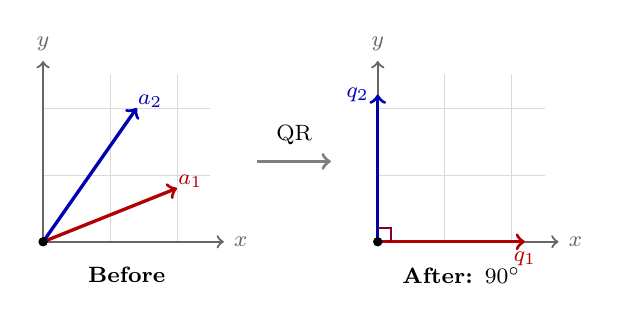
\begin{tikzpicture}[scale=0.85]
    % BEFORE: random vectors
    \begin{scope}
        \draw[very thin, black!15] (0,0) grid (2.5,2.5);
        \draw[->, thick, black!60] (0,0) -- (2.7,0) node[right, font=\footnotesize] {$x$};
        \draw[->, thick, black!60] (0,0) -- (0,2.7) node[above, font=\footnotesize] {$y$};

        \draw[->, very thick, red!70!black] (0,0) -- (2,0.8);
        \node[red!70!black, font=\footnotesize] at (2.2,0.9) {$\vect{a}_1$};
        \draw[->, very thick, blue!70!black] (0,0) -- (1.4,2);
        \node[blue!70!black, font=\footnotesize] at (1.6,2.1) {$\vect{a}_2$};

        \fill[black] (0,0) circle (2pt);
        \node[font=\footnotesize\bfseries] at (1.25,-0.5) {Before};
    \end{scope}

    % Arrow
    \draw[->, very thick, black!50] (3.2,1.2) -- (4.3,1.2);
    \node[font=\footnotesize] at (3.75,1.6) {QR};

    % AFTER: perpendicular vectors
    \begin{scope}[xshift=5cm]
        \draw[very thin, black!15] (0,0) grid (2.5,2.5);
        \draw[->, thick, black!60] (0,0) -- (2.7,0) node[right, font=\footnotesize] {$x$};
        \draw[->, thick, black!60] (0,0) -- (0,2.7) node[above, font=\footnotesize] {$y$};

        \draw[->, very thick, red!70!black] (0,0) -- (2.2,0);
        \node[red!70!black, font=\footnotesize] at (2.2,-0.25) {$\vect{q}_1$};
        \draw[->, very thick, blue!70!black] (0,0) -- (0,2.2);
        \node[blue!70!black, font=\footnotesize] at (-0.3,2.2) {$\vect{q}_2$};

        % Right angle marker
        \draw[purple!70!black, thick] (0.2,0) -- (0.2,0.2) -- (0,0.2);

        \fill[black] (0,0) circle (2pt);
        \node[font=\footnotesize\bfseries] at (1.25,-0.5) {After: $90^\circ$};
    \end{scope}
\end{tikzpicture}
\end{center}
\vspace{0.3cm}

\textbf{Why is perpendicular so great?}

Think about directions:
\begin{itemize}
    \item \textbf{Perpendicular (orthogonal):} "Go north, then go east." These are independent—going north doesn't affect your east-west position at all!
    \item \textbf{Not perpendicular:} "Go northeast, then go east-northeast." Uh, wait, how much overlap is there? This is confusing!
\end{itemize}

Perpendicular directions are \textit{independent}. They don't interfere with each other. This makes everything simpler!

\begin{definition}{QR Decomposition}{}
For any matrix $\mat{A} \in \R^{m \times n}$ (doesn't even need to be square!):
\[
\mat{A} = \mat{Q}\mat{R}
\]

where:
\begin{itemize}
    \item $\mat{Q}$ is \textbf{orthogonal}: $\mat{Q}^\top\mat{Q} = \mat{I}$ (columns are perpendicular unit vectors)
    \item $\mat{R}$ is \textbf{upper triangular} (zeros below diagonal)
\end{itemize}

\textbf{In plain English:} Take the columns of $\mat{A}$, make them perpendicular (that's $\mat{Q}$), and keep track of how to get back to the original (that's $\mat{R}$).
\end{definition}

\subsection{The Gram-Schmidt Process: A Recipe for Orthogonalization}

The algorithm to find $\mat{Q}$ is called \textbf{Gram-Schmidt}, named after Jørgen Pedersen Gram and Erhard Schmidt. (Mathematicians get to put their names on things they discover. It's a perk of the job.)

The idea is simple:
\begin{enumerate}
    \item Take the first vector. Normalize it (make it length 1). Done!
    \item Take the second vector. Remove any part that points in the first vector's direction. Normalize. Done!
    \item Take the third vector. Remove any parts that point in the first or second directions. Normalize. Done!
    \item Keep going until you've processed all vectors.
\end{enumerate}

It's like cleaning your room by picking one direction and putting away everything in that direction first, then the next direction, and so on.

\begin{example}
Let's QR decompose:
\[
\mat{A} = \begin{bmatrix}
1 & 1 \\
1 & 0 \\
0 & 1
\end{bmatrix}
\]

This has two columns (vectors in 3D space). We'll make them perpendicular.

\textbf{Step 1: First column becomes first $\mat{Q}$ column}

Our first column is $\vect{a}_1 = \begin{bmatrix} 1 \\ 1 \\ 0 \end{bmatrix}$

Its length is $\|\vect{a}_1\| = \sqrt{1^2 + 1^2 + 0^2} = \sqrt{2}$

Normalize it (make length 1):
\[
\vect{q}_1 = \frac{1}{\sqrt{2}} \begin{bmatrix} 1 \\ 1 \\ 0 \end{bmatrix} = \begin{bmatrix} 1/\sqrt{2} \\ 1/\sqrt{2} \\ 0 \end{bmatrix}
\]

\textbf{Step 2: Make second column perpendicular to first}

Our second column is $\vect{a}_2 = \begin{bmatrix} 1 \\ 0 \\ 1 \end{bmatrix}$

First, find how much of $\vect{a}_2$ points in the $\vect{q}_1$ direction (the "projection"):
\[
\text{projection} = (\vect{a}_2 \cdot \vect{q}_1) \vect{q}_1 = \left(\frac{1}{\sqrt{2}} \cdot 1 + \frac{1}{\sqrt{2}} \cdot 0 + 0 \cdot 1\right) \vect{q}_1 = \frac{1}{\sqrt{2}} \vect{q}_1
\]

Subtract the projection to get the perpendicular part:
\[
\vect{u}_2 = \vect{a}_2 - \frac{1}{\sqrt{2}} \vect{q}_1 = \begin{bmatrix} 1 \\ 0 \\ 1 \end{bmatrix} - \frac{1}{\sqrt{2}} \cdot \begin{bmatrix} 1/\sqrt{2} \\ 1/\sqrt{2} \\ 0 \end{bmatrix} = \begin{bmatrix} 1 \\ 0 \\ 1 \end{bmatrix} - \begin{bmatrix} 1/2 \\ 1/2 \\ 0 \end{bmatrix} = \begin{bmatrix} 1/2 \\ -1/2 \\ 1 \end{bmatrix}
\]

Now normalize:
\[
\|\vect{u}_2\| = \sqrt{(1/2)^2 + (-1/2)^2 + 1^2} = \sqrt{1/4 + 1/4 + 1} = \sqrt{3/2}
\]

\[
\vect{q}_2 = \frac{1}{\sqrt{3/2}} \begin{bmatrix} 1/2 \\ -1/2 \\ 1 \end{bmatrix} = \begin{bmatrix} 1/\sqrt{6} \\ -1/\sqrt{6} \\ 2/\sqrt{6} \end{bmatrix}
\]

\textbf{Verify they're perpendicular:}
\[
\vect{q}_1 \cdot \vect{q}_2 = \frac{1}{\sqrt{2}} \cdot \frac{1}{\sqrt{6}} + \frac{1}{\sqrt{2}} \cdot \frac{-1}{\sqrt{6}} + 0 \cdot \frac{2}{\sqrt{6}} = \frac{1}{\sqrt{12}} - \frac{1}{\sqrt{12}} + 0 = 0 \quad \checkmark
\]

Perpendicular! (Dot product = 0 means perpendicular. It's like a test!)

\textbf{Step 3: Build $\mat{Q}$ and $\mat{R}$}

\[
\mat{Q} = \begin{bmatrix}
1/\sqrt{2} & 1/\sqrt{6} \\
1/\sqrt{2} & -1/\sqrt{6} \\
0 & 2/\sqrt{6}
\end{bmatrix}
\]

$\mat{R}$ contains the projection coefficients and norms:
\[
\mat{R} = \begin{bmatrix}
\sqrt{2} & 1/\sqrt{2} \\
0 & \sqrt{3/2}
\end{bmatrix}
\]

(The diagonal entries are the lengths before normalizing. The off-diagonal entries are the projection coefficients.)
\end{example}

\begin{intuition}
\textbf{The Shadow Analogy}

Here's a nice way to think about Gram-Schmidt:

Imagine $\vect{q}_1$ is a flagpole sticking straight up. Now you shine a light from directly above $\vect{a}_2$. The shadow of $\vect{a}_2$ on the ground is the part that's aligned with $\vect{q}_1$.

What's left—the part that sticks up from the shadow—is $\vect{q}_2$. It's whatever wasn't captured by $\vect{q}_1$!

Each new vector is what's "new" after accounting for all previous directions.
\end{intuition}

\subsection{Why Orthogonal Matrices Are Magical}

Orthogonal matrices ($\mat{Q}$) have superpowers:

\textbf{Superpower 1: Free inverses!}

For most matrices, computing the inverse is expensive (about $n^3$ operations). But for orthogonal matrices:
\[
\mat{Q}^{-1} = \mat{Q}^\top
\]

That's it! Just flip across the diagonal. No computation needed. It's like getting a free dessert.

\textbf{Superpower 2: Length preservation!}

When you multiply a vector by $\mat{Q}$:
\[
\|\mat{Q}\vect{x}\| = \|\vect{x}\|
\]

The length stays the same! $\mat{Q}$ is a \textbf{rotation} (possibly with reflection). It spins things around but doesn't stretch or squish.

This is huge for numerical stability. Rounding errors can grow and shrink vectors, causing chaos. But orthogonal matrices are perfectly stable!

\textbf{Superpower 3: Condition number = 1}

The "condition number" measures how much small errors get amplified. For orthogonal matrices, it's exactly 1—the best possible. No error amplification!

\begin{connection}
\textbf{QR in machine learning:}

\textbf{1. Least squares (linear regression):} Fitting a line to data means solving $\mat{A}\vect{x} \approx \vect{b}$. QR gives the most numerically stable solution. If you're ever getting weird numbers from linear regression, switching to QR-based solvers often fixes it!

\textbf{2. Computing eigenvalues:} The ``QR algorithm'' repeatedly applies QR decomposition to find eigenvalues. It's a cornerstone of numerical linear algebra!

\textbf{3. Orthogonal neural networks:} Some architectures constrain weight matrices to be orthogonal to prevent gradient vanishing/exploding. They maintain orthogonality using QR!

\textbf{4. Transformers and attention:} While attention doesn't directly use QR, the idea of normalizing vectors before computing attention is the same spirit.

\textbf{5. Optimization on manifolds:} When weights must be orthogonal (helps generalization), QR is your friend!
\end{connection}

\section{Rank Factorization: The Low-Rank Art}

\subsection{Most Matrices Are Secretly Simpler Than They Look}

Here's a profound observation that powers modern AI efficiency:

\textbf{A 1000×1000 matrix has a million entries. But what if it only has rank 10?}

That means all its information actually lives in a tiny 10-dimensional subspace! The other 990 dimensions are redundant—just linear combinations of the first 10.

\textbf{Analogy time!}

Imagine a 4K ultra-HD movie file. Massive, right? Gigabytes of data!

But what if the entire movie is just a person talking in front of a gray wall? The background never changes. The person barely moves. There's almost no variation!

You could compress this movie down to almost nothing because there's not much actual \textit{information}. That's what "low rank" means for matrices—there's not as much information as the size suggests.

\vspace{0.3cm}
\begin{center}
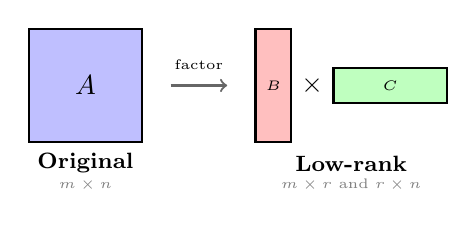
\begin{tikzpicture}[scale=0.9]
    % Original large matrix
    \draw[thick, fill=blue!25] (0,0) rectangle (1.6,1.6);
    \node at (0.8,0.8) {$\mat{A}$};
    \node[font=\footnotesize\bfseries] at (0.8,-0.3) {Original};
    \node[font=\tiny, gray] at (0.8,-0.6) {$m \times n$};

    % Arrow
    \draw[->, thick, black!60] (2,0.8) -- (2.8,0.8);
    \node[font=\tiny] at (2.4,1.1) {factor};

    % Low-rank factorization
    \begin{scope}[xshift=3.2cm]
        % B matrix (tall skinny)
        \draw[thick, fill=red!25] (0,0) rectangle (0.5,1.6);
        \node at (0.25,0.8) {\tiny $\mat{B}$};

        \node at (0.8,0.8) {$\times$};

        % C matrix (short wide)
        \draw[thick, fill=green!25] (1.1,0.55) rectangle (2.7,1.05);
        \node at (1.9,0.8) {\tiny $\mat{C}$};

        \node[font=\footnotesize\bfseries] at (1.35,-0.3) {Low-rank};
        \node[font=\tiny, gray] at (1.35,-0.6) {$m \times r$ and $r \times n$};
    \end{scope}
\end{tikzpicture}
\end{center}
\vspace{0.3cm}

\textbf{Let's do the math with real numbers:}

For a $4096 \times 4096$ matrix:
\begin{itemize}
    \item \textbf{Full storage:} $4096 \times 4096 = 16{,}777{,}216$ numbers
    \item \textbf{Rank-64 storage:} $4096 \times 64 + 64 \times 4096 = 262{,}144 + 262{,}144 = 524{,}288$ numbers
    \item \textbf{Compression ratio:} $16{,}777{,}216 / 524{,}288 = 32\times$ smaller!
\end{itemize}

And if we use rank-8 instead of rank-64? The compression ratio becomes $256\times$!

This is why LoRA (Low-Rank Adaptation) can fine-tune ChatGPT on your laptop. You're not storing millions of parameters—just thousands.

\begin{definition}{Low-Rank Factorization}{}
A matrix $\mat{A} \in \R^{m \times n}$ with rank $r$ can be written as:
\[
\mat{A} = \mat{B}\mat{C}
\]

where $\mat{B} \in \R^{m \times r}$ (tall and skinny) and $\mat{C} \in \R^{r \times n}$ (short and wide).

\textbf{Storage savings:}
\begin{itemize}
    \item Full matrix: $m \times n$ numbers
    \item Factored form: $m \times r + r \times n = r(m + n)$ numbers
\end{itemize}

If $r \ll \min(m,n)$, this is a MASSIVE savings!

\textbf{Memory formula:} Savings factor = $\frac{mn}{r(m+n)}$

For $m = n = 4096$ and $r = 8$: Savings = $\frac{4096^2}{8 \times 8192} = 256\times$
\end{definition}

\subsection{A Simple Example: The Rank-1 Matrix}

Let's see the most extreme case: a rank-1 matrix.

\begin{example}
Consider:
\[
\mat{A} = \begin{bmatrix}
1 & 2 & 3 \\
2 & 4 & 6 \\
3 & 6 & 9
\end{bmatrix}
\]

Look closely. Notice anything?

\begin{itemize}
    \item Row 2 = 2 × Row 1
    \item Row 3 = 3 × Row 1
\end{itemize}

Every row is just a scaled version of the first row! This matrix is "secretly" very simple—it's rank 1.

We can factor it as:
\[
\mat{A} = \begin{bmatrix} 1 \\ 2 \\ 3 \end{bmatrix} \begin{bmatrix} 1 & 2 & 3 \end{bmatrix} = \vect{u}\vect{v}^\top
\]

\textbf{Storage comparison:}
\begin{itemize}
    \item Full matrix: 9 numbers
    \item Factored: 3 + 3 = 6 numbers (33\% savings)
\end{itemize}

"Big deal," you say, "I saved 3 numbers."

Okay, but what about a $1000 \times 1000$ rank-1 matrix?
\begin{itemize}
    \item Full matrix: 1,000,000 numbers
    \item Factored: 1,000 + 1,000 = 2,000 numbers
    \item \textbf{Savings: 99.8\%!!!}
\end{itemize}

Now THAT's compression!
\end{example}

\begin{intuition}
\textbf{Why does rank-1 mean "one pattern"?}

A rank-1 matrix is an "outer product" of two vectors. Every element is just $a_{ij} = u_i \cdot v_j$.

Think of it like a multiplication table! The 3×3 matrix where every entry is the product of its row and column numbers:

\[
\begin{bmatrix}
1 \times 1 & 1 \times 2 & 1 \times 3 \\
2 \times 1 & 2 \times 2 & 2 \times 3 \\
3 \times 1 & 3 \times 2 & 3 \times 3
\end{bmatrix}
= \begin{bmatrix}
1 & 2 & 3 \\
2 & 4 & 6 \\
3 & 6 & 9
\end{bmatrix}
\]

It looks like 9 independent numbers, but it's really just 2 patterns (rows and columns) multiplied together!
\end{intuition}

\subsection{Low-Rank Approximation: When Close Enough Is Good Enough}

Real matrices usually aren't exactly low-rank. But they might be \textit{approximately} low-rank!

If most of the "energy" of a matrix is concentrated in a few dimensions, we can throw away the rest and barely notice.

\textbf{The SVD connection:} Remember SVD from Chapter 2?
\[
\mat{A} = \mat{U}\mat{\Sigma}\mat{V}^\top = \sum_{i=1}^r \sigma_i \vect{u}_i \vect{v}_i^\top
\]

This writes $\mat{A}$ as a sum of rank-1 matrices, weighted by singular values $\sigma_i$.

\textbf{The key insight:} Singular values are ordered from largest to smallest: $\sigma_1 \geq \sigma_2 \geq \ldots \geq \sigma_r$

If $\sigma_1 = 100$ and $\sigma_{10} = 0.001$, then the first few terms carry almost all the information!

\textbf{Approximation:} Keep only the $k$ largest singular values:
\[
\mat{A}_k = \sum_{i=1}^k \sigma_i \vect{u}_i \vect{v}_i^\top \approx \mat{A}
\]

\textbf{Error:} The approximation error is exactly $\sigma_{k+1}$—the first singular value you dropped.

If $\sigma_{k+1}$ is tiny, you lost almost nothing!

\begin{example}
\textbf{Image compression example:}

A 1024×1024 grayscale image = 1 million pixels.

But after SVD, suppose the singular values are:
\begin{itemize}
    \item $\sigma_1 = 5000, \sigma_2 = 4500, \ldots, \sigma_{50} = 100$
    \item $\sigma_{51} = 2, \sigma_{52} = 1.8, \ldots, \sigma_{1024} = 0.001$
\end{itemize}

The first 50 singular values are big; the rest are tiny!

Keep only rank 50:
\begin{itemize}
    \item Original: 1,048,576 numbers
    \item Rank-50: $1024 \times 50 + 50 \times 1024 = 102,400$ numbers
    \item Compression: 10× smaller!
    \item Visual quality: Probably indistinguishable to humans
\end{itemize}

This is basically how JPEG works (with some technical differences)!
\end{example}

\subsection{LoRA: The Revolutionary Application}

Now we get to the really exciting part—how low-rank factorization is revolutionizing AI!

\begin{connection}
\textbf{LoRA: Low-Rank Adaptation for LLMs}

This is THE technique for fine-tuning giant language models efficiently. It's why you can fine-tune LLaMA on your laptop!

\textbf{The problem:} GPT-3 has 175 billion parameters. Fine-tuning all of them requires:
\begin{itemize}
    \item Massive GPU memory (to store all gradients)
    \item Tons of compute time
    \item Lots of money
\end{itemize}

Fine-tuning all parameters is like renovating every room in a mansion when you just wanted a new bathroom.

\textbf{LoRA's brilliant insight:} Most of the weight update during fine-tuning is \textit{low-rank}!

You don't need to change everything—just a few key directions in weight space. It's like the model saying: "I already know how to speak English. I just need small adjustments to sound like a pirate. Arrr!"

\textbf{How it works:}

Instead of updating $\mat{W}$ directly, learn a low-rank update:
\[
\mat{W}_{\text{new}} = \mat{W}_{\text{original}} + \Delta\mat{W} = \mat{W}_{\text{original}} + \mat{B}\mat{A}
\]

where:
\begin{itemize}
    \item $\mat{W}_{\text{original}}$ is frozen (don't touch!)
    \item $\mat{B} \in \R^{d \times r}$ is a skinny matrix (trained)
    \item $\mat{A} \in \R^{r \times d}$ is a short matrix (trained)
    \item $r \ll d$ (like $r = 8$ when $d = 4096$)
\end{itemize}

\vspace{0.3cm}
\begin{center}
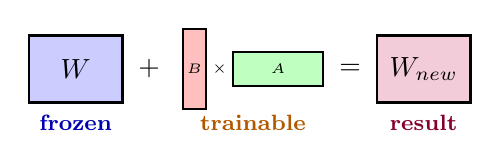
\begin{tikzpicture}[scale=0.85]
    % Original W (frozen)
    \draw[thick, fill=blue!20] (0,0) rectangle (1.4,1);
    \node at (0.7,0.5) {$\mat{W}$};
    \node[font=\footnotesize\bfseries, blue!70!black] at (0.7,-0.3) {frozen};

    \node at (1.8,0.5) {$+$};

    % LoRA update: B x A
    \begin{scope}[xshift=2.3cm]
        % B matrix (tall skinny)
        \draw[thick, fill=red!25] (0,-0.1) rectangle (0.35,1.1);
        \node[font=\tiny] at (0.175,0.5) {$\mat{B}$};

        \node[font=\tiny] at (0.55,0.5) {$\times$};

        % A matrix (short wide)
        \draw[thick, fill=green!25] (0.75,0.25) rectangle (2.1,0.75);
        \node[font=\tiny] at (1.425,0.5) {$\mat{A}$};

        \node[font=\footnotesize\bfseries, orange!70!black] at (1.05,-0.3) {trainable};
    \end{scope}

    \node at (4.8,0.5) {$=$};

    % Result
    \draw[thick, fill=purple!20] (5.2,0) rectangle (6.6,1);
    \node at (5.9,0.5) {$\mat{W}_{\text{new}}$};
    \node[font=\footnotesize\bfseries, purple!70!black] at (5.9,-0.3) {result};
\end{tikzpicture}
\end{center}
\vspace{0.3cm}

\textbf{The numbers are mind-blowing:}

\begin{center}
\begin{tabular}{|l|r|r|}
\hline
\textbf{Method} & \textbf{Parameters} & \textbf{Savings} \\
\hline
Full fine-tuning (4096×4096) & 16,777,216 & — \\
LoRA rank 64 & 524,288 & 32× \\
LoRA rank 16 & 131,072 & 128× \\
LoRA rank 8 & 65,536 & 256× \\
LoRA rank 4 & 32,768 & 512× \\
\hline
\end{tabular}
\end{center}

With rank 8, you're training 256× fewer parameters! And the crazy thing? \textbf{It usually works just as well!}

\textbf{Why does LoRA work so well?}

The key insight is that fine-tuning doesn't need to change everything—it just needs to adjust a few key directions.

Think of it like this: GPT-3 already knows how to write English. Fine-tuning for customer service just means: "Be polite. Refer to our products. End with 'How else can I help?'" That's not a complete rewrite—it's a few tweaks!

Mathematically, the "intrinsic dimensionality" of the fine-tuning task is low. The model's weights live in a 175-billion-dimensional space, but the useful updates only span maybe 64 dimensions. LoRA exploits this!
\end{connection}

\section{Putting It All Together: The Decomposition Toolkit}

\subsection{Which Decomposition Should I Use?}

Here's your ultimate cheat sheet. Print it out. Tattoo it on your arm. Whatever works!

\begin{center}
\small
\resizebox{\textwidth}{!}{%
\begin{tabular}{|l|l|l|l|}
\hline
\textbf{Decomposition} & \textbf{When to Use} & \textbf{Superpower} & \textbf{Vibe} \\
\hline
Cholesky & Symmetric positive definite & Fastest solver, stable & Square root \\
\hline
LU & Square matrices, many solves & Factor once, solve many & Elimination \\
\hline
QR & Least squares problems & Most numerically stable & Perpendicular \\
\hline
SVD & Any matrix, low-rank approx & Swiss army knife & The GOAT \\
\hline
Eigen & Square, understanding dynamics & See stretches \& rotations & Diagonal \\
\hline
Low-rank & Compression, LoRA & Massive storage savings & Less is more \\
\hline
\end{tabular}%
}
\end{center}

\subsection{Quick Decision Tree}

Confused about which decomposition to use? Follow this!

\begin{enumerate}
    \item \textbf{Is the matrix symmetric positive definite?} (Covariance? Hessian?)
    \begin{itemize}
        \item Yes \textrightarrow{} \textbf{Cholesky}. Don't think, just do it.
    \end{itemize}

    \item \textbf{Are you solving $\mat{A}\vect{x} = \vect{b}$ for many different $\vect{b}$?}
    \begin{itemize}
        \item Yes \textrightarrow{} \textbf{LU} (or Cholesky if symmetric PD)
    \end{itemize}

    \item \textbf{Are you doing least squares / linear regression?}
    \begin{itemize}
        \item Yes \textrightarrow{} \textbf{QR}. It's the most stable.
    \end{itemize}

    \item \textbf{Do you need a low-rank approximation?}
    \begin{itemize}
        \item Yes \textrightarrow{} \textbf{SVD} (gives the best approximation!)
    \end{itemize}

    \item \textbf{Do you need to compress or adapt a neural network?}
    \begin{itemize}
        \item Yes \textrightarrow{} \textbf{Low-rank factorization} (LoRA style!)
    \end{itemize}

    \item \textbf{Do you want to understand the geometry (stretches, rotations)?}
    \begin{itemize}
        \item Yes \textrightarrow{} \textbf{SVD} or \textbf{Eigendecomposition}
    \end{itemize}
\end{enumerate}

\subsection{The Grand Philosophy}

All these decompositions share one beautiful philosophy:

\begin{center}
\textit{\Large "Break complex things into simple, interpretable pieces."}
\end{center}

\vspace{0.3cm}

Each decomposition has its own flavor of simplicity:

\begin{itemize}
    \item \textbf{Cholesky:} "This positive definite matrix is just a lower triangular matrix times its reflection!"
    \item \textbf{LU:} "Any matrix is just lower triangular × upper triangular. Elimination packaged neatly!"
    \item \textbf{QR:} "Any matrix is just a rotation × upper triangular. Perpendicularity achieved!"
    \item \textbf{SVD:} "Any matrix is just rotation × stretch × rotation. The ultimate breakdown!"
    \item \textbf{Eigen:} "Square matrices stretch along their eigenvectors. That's it!"
    \item \textbf{Low-rank:} "This huge matrix is secretly just two skinny matrices having a conversation."
\end{itemize}

Once you see the pieces, you can:
\begin{itemize}
    \item \textbf{Understand:} "Oh, it's mostly stretching 5× in this direction!"
    \item \textbf{Compute:} "I can work with triangular matrices WAY faster!"
    \item \textbf{Compress:} "I only need 64 dimensions, not 4096!"
    \item \textbf{Adapt:} "I'll update just this tiny low-rank part!"
    \item \textbf{Debug:} "The condition number is huge because of that one tiny singular value..."
\end{itemize}

\section{Practice Problems (With Hints!)}

Time to test your understanding! Don't worry—these are designed to be doable, not traumatic.

\subsection{Problem 1: Cholesky Decomposition (Warm-up)}

Find the Cholesky decomposition of:
\[
\mat{A} = \begin{bmatrix}
9 & 6 \\
6 & 5
\end{bmatrix}
\]

\textbf{Hints:}
\begin{itemize}
    \item Start with $\ell_{11} = \sqrt{9} = 3$
    \item Then find $\ell_{21}$ from the off-diagonal
    \item Finally find $\ell_{22}$ from the bottom-right
\end{itemize}

\subsection{Problem 2: Understanding Rank (Conceptual)}

A matrix $\mat{W} \in \R^{1024 \times 1024}$ has rank 16.

\begin{enumerate}
    \item How many numbers to store the full matrix?
    \item How many numbers if stored as $\mat{W} = \mat{B}\mat{C}$ where $\mat{B} \in \R^{1024 \times 16}$ and $\mat{C} \in \R^{16 \times 1024}$?
    \item What's the compression ratio?
    \item \textbf{Bonus:} Why might real neural network weights be approximately low-rank?
\end{enumerate}

\textbf{Hint:} Just multiply dimensions!

\subsection{Problem 3: LoRA Math (Applied)}

You're fine-tuning a language model. One weight matrix is $4096 \times 4096$.

\begin{enumerate}
    \item Full fine-tuning: How many parameters?
    \item LoRA with rank $r=4$: How many parameters?
    \item LoRA with rank $r=64$: How many parameters?
    \item \textbf{Challenge:} At what rank $r$ does LoRA stop saving memory compared to full fine-tuning?
\end{enumerate}

\textbf{Hint for part 4:} Set $r(m+n) = mn$ and solve for $r$.

\subsection{Problem 4: Decomposition Choice (Practical)}

For each scenario, which decomposition would you choose? Explain briefly.

\begin{enumerate}
    \item Sampling random points from a multivariate Gaussian distribution
    \item Finding the principal components of a dataset
    \item Solving 100 systems $\mat{A}\vect{x}_i = \vect{b}_i$ with the same $\mat{A}$ (and $\mat{A}$ is symmetric positive definite)
    \item Compressing a neural network weight matrix to 10\% of its original size
    \item Checking if a covariance matrix is valid (positive semi-definite)
\end{enumerate}

\subsection{Problem 5: Low-Rank Intuition (Thought Experiment)}

Consider these two 1000×1000 matrices:

\textbf{Matrix A:} Each row is just a random permutation of the numbers 1 to 1000.

\textbf{Matrix B:} Each row is the first row multiplied by some random scalar.

\begin{enumerate}
    \item What's the rank of Matrix A? (Probably?)
    \item What's the rank of Matrix B?
    \item Which one compresses better?
    \item What real-world data might look like Matrix B?
\end{enumerate}

\section{Key Takeaways}

Let's summarize what you've learned! These are the big ideas:

\begin{enumerate}
    \item \textbf{Decompositions break matrices into simpler pieces}---triangular, orthogonal, diagonal, or low-rank.

    \item \textbf{Cholesky} ($\mat{A} = \mat{L}\mat{L}^\top$) is the ``matrix square root'' for symmetric positive definite matrices.

    \item \textbf{LU} ($\mat{A} = \mat{L}\mat{U}$) packages Gaussian elimination. Factor once, solve many systems!

    \item \textbf{QR} ($\mat{A} = \mat{Q}\mat{R}$) finds perpendicular directions. Most stable for least squares!

    \item \textbf{Low-rank factorization} ($\mat{A} \approx \mat{B}\mat{C}$) is the secret to compression.

    \item \textbf{LoRA uses low-rank updates} to fine-tune LLMs with 100-256× fewer parameters. This is why you can fine-tune on consumer hardware!

    \item \textbf{The philosophy:} Don't fight complexity head-on. Break it into pieces, understand each piece, then reassemble.
\end{enumerate}

\begin{connection}
\textbf{The Deep Learning Connection: A Summary}

Everything we learned connects directly to modern AI:

\textbf{During Training:}
\begin{itemize}
    \item Eigenvalues of the Hessian tell you about the optimization landscape
    \item Cholesky factors help with natural gradient and second-order methods
    \item Low-rank structure in gradients enables efficient distributed training
\end{itemize}

\textbf{During Inference:}
\begin{itemize}
    \item Low-rank approximations speed up matrix multiplications
    \item Quantization (related to low-rank ideas) shrinks model size
    \item Structured matrices (triangular, orthogonal) enable faster computation
\end{itemize}

\textbf{For Fine-tuning:}
\begin{itemize}
    \item LoRA makes adaptation accessible to everyone
    \item QLoRA combines low-rank with quantization for even smaller footprints
    \item Adapter methods use low-rank insertions throughout the network
\end{itemize}

\textbf{For Understanding:}
\begin{itemize}
    \item SVD of weight matrices reveals what features the model learned
    \item Eigenanalysis of attention patterns shows what the model "looks at"
    \item Low-rank structure in representations suggests compressed knowledge
\end{itemize}

\textbf{The meta-lesson:} Every breakthrough in making LLMs practical—faster, smaller, more adaptable—relies on clever use of matrix decompositions.

When you hear about a new AI efficiency technique, ask yourself: "What decomposition is this exploiting?" You'll usually find one hiding in there!
\end{connection}

\vspace{0.5cm}

\begin{center}
\fbox{\parbox{0.85\textwidth}{
\centering
\large\textbf{ Congratulations! }

\vspace{0.3cm}

You now understand matrix decompositions—the secret weapons of efficient AI!

\vspace{0.3cm}

\normalsize
You can explain:
\begin{itemize}
    \item Why Cholesky is like taking a matrix square root
    \item How LU packages Gaussian elimination for reuse
    \item Why perpendicular directions (QR) are numerically magical
    \item How low-rank factorization enables 256× parameter savings in LoRA
\end{itemize}

\vspace{0.3cm}

\textbf{That's seriously impressive. Most people never learn this!}
}}
\end{center}

\vspace{0.5cm}

\begin{center}
\large\textit{Next up: Calculus—the mathematics of change and optimization!}

\vspace{0.3cm}

\normalsize
(Where we'll learn how neural networks actually learn by following gradients down the loss landscape. Spoiler: It's like rolling a ball down a bowl... a very high-dimensional bowl!)
\end{center}
